\section{Mathematical Formulation}
\label{sec:mathematical_formulation}

ManiGit establishes a formal mathematical separation between \textit{memory storage} and \textit{context compilation}. While memory storage $\mathcal{M}_t$ accumulates monotonically across an agent's lifecycle, the operative context window $C_t$ assembled for query $q_t$ must respect a strict token budget $B$. Fig.~\ref{fig:context_compilation} illustrates the budget-constrained context selection problem.

\begin{figure}[t]
\centering
\resizebox{0.98\columnwidth}{!}{%
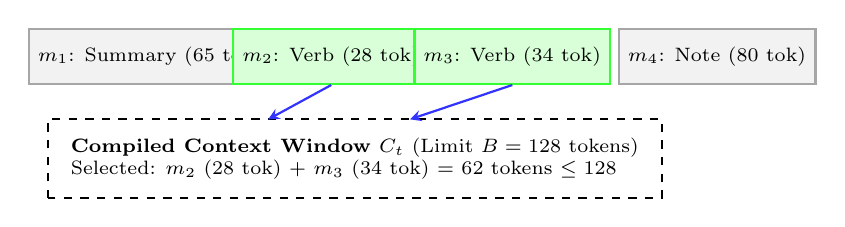
\begin{tikzpicture}[
    item/.style={rectangle, draw=gray!70, fill=gray!10, thick, minimum height=0.7cm, align=center, font=\scriptsize},
    active/.style={rectangle, draw=green!80, fill=green!15, thick, minimum height=0.7cm, align=center, font=\scriptsize},
    flow/.style={->, >=stealth, thick, color=blue!80}]

\node[item, minimum width=2.2cm] (m1) {$m_1$: Summary (65 tok)};
\node[active, minimum width=1.5cm, right of=m1, xshift=1.3cm] (m2) {$m_2$: Verb (28 tok)};
\node[active, minimum width=1.8cm, right of=m2, xshift=1.3cm] (m3) {$m_3$: Verb (34 tok)};
\node[item, minimum width=2.5cm, right of=m3, xshift=1.6cm] (m4) {$m_4$: Note (80 tok)};

\draw[draw=black, dashed, thick] (-1.3, -1.8) rectangle (6.5, -0.8);
\node[font=\scriptsize, align=left] at (2.6, -1.3) {\textbf{Compiled Context Window $C_t$} (Limit $B=128$ tokens)\\Selected: $m_2$ (28 tok) + $m_3$ (34 tok) = 62 tokens $\le 128$};

\draw[flow] (m2.south) -- (1.5, -0.8);
\draw[flow] (m3.south) -- (3.3, -0.8);

\end{tikzpicture}%
}

\caption{Mathematical knapsack formulation of context compilation. Memory objects are ranked by utility density $D(m_i,q_t)=U(m_i,q_t)/L(m_i)$ and selected under the hard token budget $B$.}
\label{fig:context_compilation}
\end{figure}

\subsection{Formal Optimization Problem}
Let $\mathcal{M}_t = \{m_1, m_2, \dots, m_N\}$ be the set of active memory objects in the current branch at turn $t$. Each memory object $m_i$ possesses:
\begin{itemize}
    \item A token length $L(m_i) \in \mathbb{N}^+$, measured via deterministic tokenization.
    \item A functional tier $\tau(m_i) \in \{\texttt{VERBATIM}, \texttt{SUMMARY}, \texttt{ARCHIVED}, \texttt{TOMBSTONE}\}$.
    \item An intrinsic priority weight $p(m_i) \in [0, 1]$.
    \item An age or creation timestamp $t(m_i)$.
\end{itemize}

Given an incoming user query $q_t$ and a hard pre-allocated token budget $B \in \mathbb{N}^+$, the context compilation objective is to select an optimal subset $C_t^* \subseteq \mathcal{M}_t$ such that:
\begin{equation}
C_t^* = \arg\max_{C_t \subseteq \mathcal{M}_t} \sum_{m_i \in C_t} U(m_i, q_t)
\label{eq:knapsack_obj}
\end{equation}
subject to the hard budget constraint:
\begin{equation}
\sum_{m_i \in C_t} L(m_i) \le B
\label{eq:knapsack_constraint}
\end{equation}
where only active memories are eligible for selection ($\tau(m_i) \in \{\texttt{VERBATIM}, \texttt{SUMMARY}\}$).

\subsection{Composite Utility Function}
The utility $U(m_i, q_t)$ evaluates the suitability of memory $m_i$ for query $q_t$ as a convex combination of relevance, tier boost, and priority:
\begin{equation}
U(m_i, q_t) = w_{\text{rel}} \cdot R(m_i, q_t) + w_{\text{tier}} \cdot T(m_i) + w_{\text{prio}} \cdot p(m_i)
\label{eq:utility}
\end{equation}
where:
\begin{itemize}
    \item $R(m_i, q_t) \in [0, 1]$ is the normalized lexical relevance score between query $q_t$ and memory content $m_i$, computed via Okapi BM25 and term overlap:
    $$R(m_i, q_t) = \frac{\text{BM25}(m_i, q_t)}{\max_{m_j \in \mathcal{M}_t} \text{BM25}(m_j, q_t) + \epsilon}$$
    \item $T(m_i) \in [0, 1]$ is the tier-specific preference multiplier:
    $$T(m_i) = \begin{cases}
    1.0, & \text{if } \tau(m_i) = \texttt{VERBATIM} \\
    0.7, & \text{if } \tau(m_i) = \texttt{SUMMARY} \\
    0.0, & \text{otherwise}
    \end{cases}$$
    \item $p(m_i) \in [0, 1]$ is the intrinsic priority assigned during intake (e.g., $1.0$ for security credentials, $0.8$ for architecture choices, $0.5$ for conversational summaries).
    \item $w_{\text{rel}} = 0.5$, $w_{\text{tier}} = 0.3$, and $w_{\text{prio}} = 0.2$ are normalized mixture weights summing to $1.0$.
\end{itemize}

\subsection{Greedy Knapsack Approximation Algorithm}
The optimization problem defined in Equations~\eqref{eq:knapsack_obj} and~\eqref{eq:knapsack_constraint} is isomorphic to the classic 0-1 Knapsack Problem, which is known to be NP-hard. ManiGit does not solve the exact combinatorial optimization problem at inference time; instead, this formulation motivates our practical system design, which uses local lexical retrieval, tier/confidence/priority scoring signals, and a deterministic greedy score-density selection algorithm:

\begin{enumerate}
    \item \textbf{Density Calculation:} For every active memory $m_i \in \mathcal{M}_t$, compute its utility density per token:
    \begin{equation}
    D(m_i, q_t) = \frac{U(m_i, q_t)}{L(m_i)}
    \end{equation}
    \item \textbf{Sorting:} Sort candidate memories in descending order of density:
    \begin{equation}
    D(m_{(1)}, q_t) \ge D(m_{(2)}, q_t) \ge \dots \ge D(m_{(N)}, q_t)
    \end{equation}
    \item \textbf{Greedy Packing:} Initialize $C_t \leftarrow \emptyset$ and accumulated tokens $K \leftarrow 0$. For each sorted candidate $m_{(i)}$:
    \begin{equation}
    \begin{aligned}
    &\text{if } K + L(m_{(i)}) \le B\text{ then} \\
    &\quad C_t \leftarrow C_t \cup \{m_{(i)}\}, \quad K \leftarrow K + L(m_{(i)})
    \end{aligned}
    \end{equation}
    \item \textbf{Early Termination:} Stop when no remaining candidate fits within the residual budget $B - K$.
\end{enumerate}

\subsection{Theoretical Guarantee: Memory $\ne$ Context}
This formulation guarantees two critical invariants:
\begin{enumerate}
    \item \textbf{Budget Invariance:} $\sum_{m_i \in C_t} L(m_i) \le B$ holds strictly for all $t$ and all queries, ensuring that agent prompts never exceed allocated token budgets or trigger LLM context overflow errors.
    \item \textbf{Decoupled Scalability:} The total size of persistent memory $|\mathcal{M}_t|$ can grow indefinitely without expanding the active context size $|C_t|$, successfully decoupling agent operational longevity from model inference cost.
\end{enumerate}
